\documentclass[a4paper,10.9pt]{article}
\usepackage[utf8]{inputenc}
\usepackage[T1]{fontenc}
\usepackage{fancyhdr} % pour personnaliser les en-têtes
\usepackage{lastpage}
\usepackage[frenchb]{babel}
\usepackage{amsfonts,amssymb}
\usepackage{amsmath,amsthm}
\usepackage{paralist}
\usepackage{xspace}
\usepackage{xcolor}
\usepackage{variations}
\usepackage{xypic}
\usepackage{eurosym,multicol}
\usepackage{graphicx}
\usepackage[np]{numprint}
\usepackage{hyperref} 
\usepackage{listings} % pour écrire des codes avec coloration syntaxique  

\usepackage{tikz}
\usetikzlibrary{calc, arrows, plotmarks,decorations.pathreplacing}
\usepackage{colortbl}
\usepackage{multirow}
\usepackage[top=1.5cm,bottom=1.5cm,right=1.5cm,left=1.5cm]{geometry}

\newtheorem{defi}{Définition}
\newtheorem{thm}{Théorème}
\newtheorem{thm-def}{Théorème/Définition}
\newtheorem{rmq}{Remarque}
\newtheorem{prop}{Propriété}
\newtheorem{cor}{Corollaire}
\newtheorem{lem}{Lemme}
\newtheorem{ex}{Exemple}
\newtheorem{cex}{Contre-exemple}
\newtheorem{prop-def}{Propriété-définition}
\newtheorem{exer}{Exercice}
\newtheorem{nota}{Notation}
\newtheorem{ax}{Axiome}
\newtheorem{appl}{Application}
\newtheorem{csq}{Conséquence}
\theoremstyle{definition}
\newtheorem{exo}{Exercice}


\newcommand{\vtab}{\rule[-0.4em]{0pt}{1.2em}}
\newcommand{\V}{\overrightarrow}
\renewcommand{\thesection}{\Roman{section} }
\renewcommand{\thesubsection}{\arabic{subsection} }
\renewcommand{\thesubsubsection}{\alph{subsubsection} }
\newcommand{\C}{\mathbb{C}}
\newcommand{\R}{\mathbb{R}}
\newcommand{\Q}{\mathbb{Q}}
\newcommand{\Z}{\mathbb{Z}}
\newcommand{\N}{\mathbb{N}}


\definecolor{vert}{RGB}{11,160,78}
\definecolor{rouge}{RGB}{255,120,120}
% Set the beginning of a LaTeX document
\pagestyle{fancy}
\begin{document}
	
\lhead{Lycée Le Maurice Genevoix}\chead{}\rhead{Année~2021-2022}\lfoot{M. Botcazou}\cfoot{\thepage/3}\rfoot{\textbf{Tourner la page S.V.P.}}\renewcommand{\headrulewidth}{0.4pt}\renewcommand{\footrulewidth}{0.4pt}

\hfill\\[-1cm]
$$	\fbox{\text{\Large{ \sc Correction du Devoir Maison rendu pour le le 03 janvier  2022 }}}$$	


\begin{exo}\textit{\textbf{Les vecteurs, des bons outils pour faire de la physique:}} 
\begin{defi}\quad\\
	\par $\bullet$ \quad Une \textbf{ force} correspond en physique à une action mécanique d'un objet sur un autre. L'unité de mesure d'une force est le \textbf{Newton}, référence au célèbre physicien britannique Isaac Newton (1643-1727).\\
	\par $\bullet$ \quad Une force qui agit sur un objet admet une \textbf{direction}, une \textbf{intensité}, un \textbf{sens} et un \textbf{point d'application}.   
\end{defi}  
\begin{prop}
	L'action des forces sur un objet peut créer du mouvement, elle peut entrainer une variation sur la vitesse de cet objet.
\end{prop}
\subsection*{Comment utiliser les vecteurs pour représenter des forces dans une situation physique?}
\noindent Une pomme est tranquillement accrochée dans un pommier, nous la regardons elle est immobile. En un instant elle se met en mouvement, elle se décroche de la branche et chute vers le sol. 
\section*{Une pomme accrochée dans un arbre :}

\textbf{QUESTIONS:}\\
\begin{enumerate}
	\item 
	 \begin{enumerate}
	 	\item Chaque gramme de la pomme est attiré vers la terre avec une force de ~0.01~ Newton.\\ 
	 	Or notre pomme pèse 120 grammes.\\
		Donc: \quad $120 \times 0.01 = 1.2$\\
	 	L'intensité de la force de gravité terrestre subie par la pomme est de $1.2$ Newton. Nous noterons $\vec{G}$ la force de gravité terrestre subie par la pomme.\\
	 	\item En s'aidant du schéma 1 donné en Annexe, nous trouvons que :\\
	 	 La direction de la force de gravité subie par la pomme est donnée par une droite, cette droite est la droite $\left(AC\right)$. Le sens de la force de gravité subie par la pomme est vers le bas.\\ \textit{(Notez que la droite } $\left(AC\right)$ \textit{peut aussi se noté comme : } $\left(AS\right)$ \textit{ou} $\left(CS\right)$ \textit{nous parlons ici de la même droite)} \\
	 \end{enumerate} 
	 
	\item \begin{enumerate}
		\item Avec l'échelle d'un carreau pour ~0.4~Newton, si la force de gravité subie par la pomme a une intensité de $1.2$ Newton, le nombre de carreaux nécessaire pour représenter la force de gravité subie par la pomme est de: \quad $1.2 \div 0.4 \ = \ 3$\\
		Donc $3$ carreaux sont nécessaires.\\
		\item Représenter sur le schéma 1 à l'aide d'un vecteur qui part du point C, la force de gravité subi par la pomme.\\ \textit{\textbf{(Attention en physique un vecteur représentant une force a un point d'accroche, on parle de point d'application. Ici ce point est le point C)}}\\ \textbf{\textit{(Voir Annexe 1)}}
	\end{enumerate}
	\item Au premier regard la pomme était immobile, cela signifie que la somme des forces subie par la pomme était nulle. Au départ, la branche exerce une force contraire qui retient la pomme. Un physicien nous dit :~~\textit{"Chaque gramme de la pomme est retenue par la branche avec une force de ~0.01~ Newton"} \\
	\begin{enumerate}
		\item Chaque gramme de la pomme est retenue par la branche avec une force de ~0.01~ Newton.\\
		Or notre pomme pèse 120 grammes.\\
		Donc: \quad $120 \times 0.01 = 1.2$\\
		L'intensité de la force de retenue de la branche sur la pomme est donc de $1.2$ Newton. Nous noterons $\vec{R}$ la force de retenue de la branche.\\
		\item En s'aidant du schéma 1 donné en Annexe, nous trouvons que :\\
		La direction de la force de retenue de la branche est donnée par une droite, cette droite est la droite $\left(AC\right)$, le sens de la force de retenue de la branche est vers le haut.\\ \textit{(Notez que la droite } $\left(AC\right)$ \textit{peut aussi se noté comme : } $\left(AS\right)$ \textit{ou} $\left(CS\right)$ \textit{nous parlons ici de la même droite)} \\
	\end{enumerate}
	\item
	 \begin{enumerate}
		\item Avec l'échelle d'un carreau pour ~0.4~Newton, si la force de retenue de la branche sur la pomme a une intensité de $1.2$ Newton, le nombre de carreaux nécessaire pour représenter la force de retenue de la branche sur la pomme est de: \quad $1.2 \div 0.4 \ = \ 3$\\
		Donc $3$ carreaux sont nécessaires.
		\item Représenter sur le schéma 1 à l'aide d'un vecteur qui part du point A, la force de retenue de la branche sur la pomme.
		\\ \textit{\textbf{(Attention en physique un vecteur représentant une force a un point d'accroche, on parle de point d'application. Ici ce point est le point A)}}\\ \textbf{\textit{(Voir Annexe 1)}}
	\end{enumerate}
	\item  Le vecteur ~$\vec{G}$~ et le vecteur ~$\vec{R}$~ ont la même direction qui est la droite $\left(AC\right)$.\\
	 Le vecteur ~$\vec{G}$~ et le vecteur ~$\vec{R}$~ ont la même norme qui est de $1.2$.\\
	  Le vecteur ~$\vec{G}$~ et le vecteur ~$\vec{R}$~ n'ont pourtant pas le même sens, le vecteur ~$\vec{G}$~ va vers le bas et le vecteur ~$\vec{R}$~ lui va vers le haut\\
	  La somme des vecteurs ~~$\vec{G} \ + \ \vec{R}$~~ est alors égale au vecteur nul : \quad~~$\vec{G} \ + \ \vec{R} \ = \ \vec{0}$~~   
\end{enumerate}
\section*{Une pomme qui chute vers le sol :}
\noindent Les fortes chaleurs de l'été et le vent fragilisent la résistance des branches. La force de retenue de la branche sur la pomme diminue en intensité avec le temps. Lorsque la sommes des forces subie par la pomme n'est plus nulle, la pomme se met en mouvement et chute vers le sol.\\

\textbf{QUESTIONS:}\\
\begin{enumerate}
	\item[6.] Notre pomme pèse toujours 120 grammes.\\
	\begin{enumerate}
		\item Chaque gramme de la pomme est toujours attiré vers la terre avec une force de ~0.01~ Newton.\\ 
		Or notre pomme pèse 120 grammes.\\
		Donc: \quad $120 \times 0.01 = 1.2$\\
		L'intensité de la force de gravité terrestre subie par la pomme est de $1.2$ Newton. Nous noterons $\vec{G}$ la force de gravité terrestre subie par la pomme.\\
		\item Avec la même échelle d'un carreau pour ~0.4~Newton, si la force de gravité terrestre subie par la pomme est de $1.2$ Newton, le nombre de carreaux nécessaire pour représenter la force de gravité subie par la pomme est de: \quad $1.2 \div 0.4 \ = \ 3$\\
		Donc $3$ carreaux sont nécessaires.
		\\ \textit{\textbf{(Attention en physique un vecteur représentant une force a un point d'accroche, on parle de point d'application. Ici ce point est le point C)}}\\ \textbf{\textit{(Voir Annexe 2)}}\\
	\end{enumerate} 
	\item[7.] Juste avant que la pomme ne tombe, un physicien nous dit : ~~\textit{"Chaque gramme de la pomme est maintenant retenue par la branche avec une force de ~0.005~ Newton"}\\ 
	\begin{enumerate}
		\item Chaque gramme de la pomme est retenue maintenant par la branche avec une force de ~0.005~ Newton.\\
		Or notre pomme pèse 120 grammes.\\
		Donc: \quad $120 \times 0.005 = 0.6$\\
		L'intensité de la force de retenue de la branche sur la pomme est maintenant  donc de $0.6$ Newton. Nous noterons $\vec{R}$ la force de retenue de la branche.\\
	
		\item Avec l'échelle d'un carreau pour ~0.4~Newton, si la force de retenue de la branche sur la pomme a une intensité de $0.6$ Newton, le nombre de carreaux nécessaire pour représenter la force de retenue de la branche sur la pomme est de: \quad $0.6 \div 0.4 \ = \ 1.5$\\
		Donc $1.5$ carreaux sont nécessaires.\
		\\ \textit{\textbf{(Attention en physique un vecteur représentant une force a un point d'accroche, on parle de point d'application. Ici ce point est le point A)}}\\ \textbf{\textit{(Voir Annexe 2)}}\\
	\end{enumerate}
	\item[8.] Le vecteur ~$\vec{G}$~ et le vecteur ~$\vec{R}$~ ont la même direction qui est la droite $\left(AC\right)$.\\
	Le vecteur ~$\vec{G}$~ et le vecteur ~$\vec{R}$~ n'ont plus la même norme. La norme du vecteur ~$\vec{G}$~ est de $1.2$ et la norme du vecteur ~$\vec{R}$~ est de $0.6$ \\
	Le vecteur ~$\vec{G}$~ et le vecteur ~$\vec{R}$~ n'ont  pas le même sens, le vecteur ~$\vec{G}$~ va vers le bas et le vecteur ~$\vec{R}$~ lui va vers le haut\\\\
	La somme des vecteurs ~~$\vec{G} \ + \ \vec{R}$~~ n'est plus égal au vecteur nul, elle est alors égale à un vecteur qui a:
	\item[-] Pour direction la droite $\left(AC\right)$
	\item[-] Pour norme $0.6$ car on sait que  $1.2 - 0.6 \ = \ 0.6$ 
	\item[-] Pour sens le bas. \\\\
	\textbf{BONUS:}\\
	\item[9.] Il existe un lien entre la somme des forces exercé sur un objet et la mise en mouvement de celui-ci.
	 \item[-]Dans la situation 1, la somme  des vecteurs forces exercée sur la pomme était nulle, notre pomme restait donc immobile.
	\item[-]Dans la situation 2, la somme  des vecteurs forces exercée sur la pomme n'est plus nulle, notre pomme est mise en mouvement et se décroche de l'arbre puis finie sa vie au sol.\\\\
	\textit{"Elle ne tombera pas plus bas"}
	
	
\end{enumerate}


\section*{ANNEXE:}
\subsection*{Annexe 1:}
\begin{figure*}[!h]
	\centering
	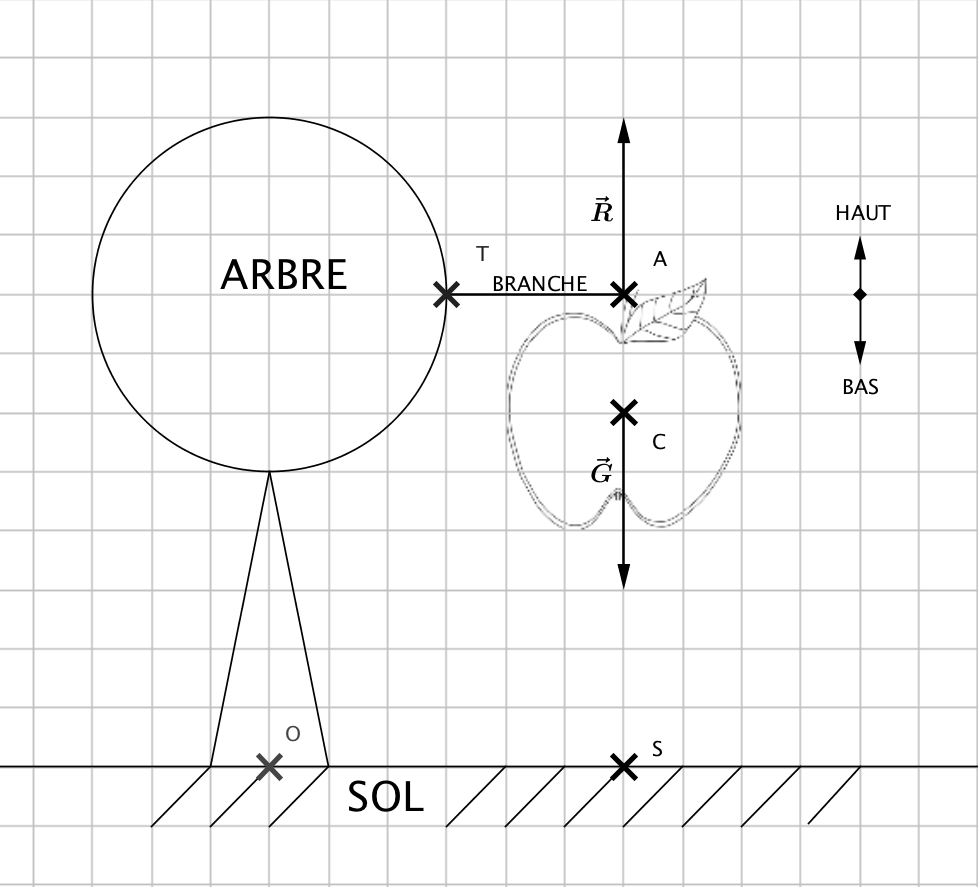
\includegraphics[scale=1]{DM_2_1.png}	
\end{figure*}
\subsection*{Annexe 2:}
\begin{figure*}[!h]
	\centering
	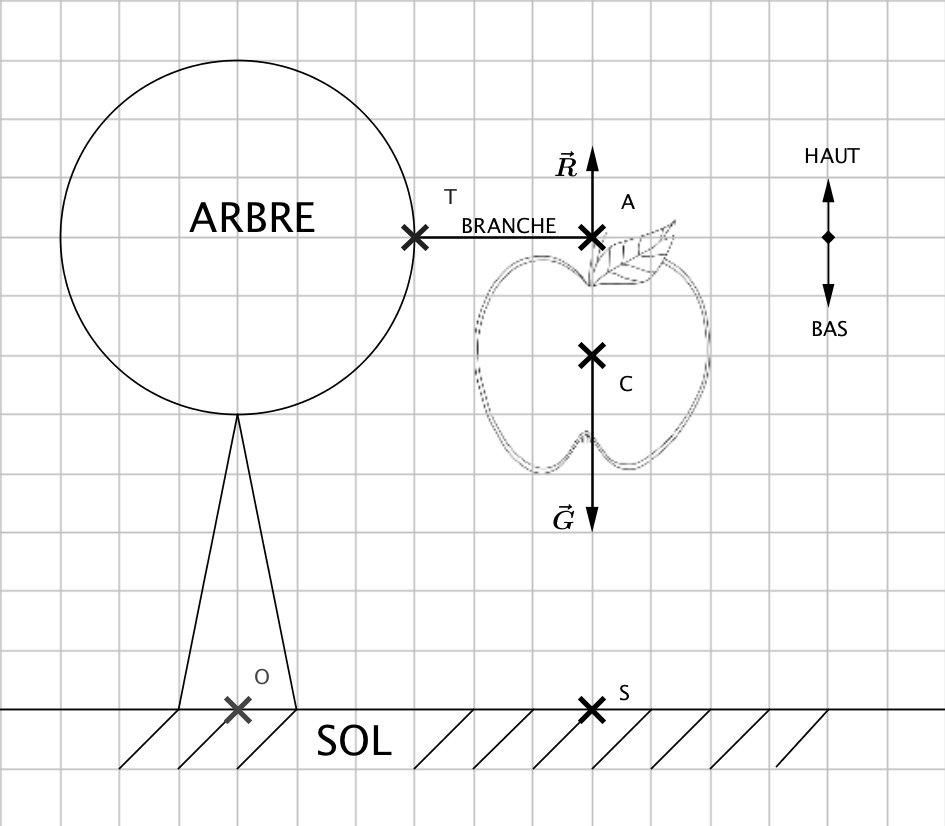
\includegraphics[scale=1]{DM_2_2.png}	
\end{figure*}
\end{exo}
\end{document}